\documentclass[a4paper]{article}
\usepackage[warn]{mathtext}
\usepackage[utf8]{inputenc}
\usepackage[T2A]{fontenc}
\usepackage[english,russian]{babel}
\usepackage{indentfirst}
\usepackage{misccorr}
\usepackage{subcaption}
\captionsetup{compatibility=false}
\usepackage{geometry}
\geometry{verbose,a4paper,tmargin=2cm,bmargin=2cm,lmargin=1.5cm,rmargin=1.5cm}
\usepackage{graphicx}
\usepackage{wrapfig}
\usepackage{amsmath}
\usepackage{fancyhdr}
\usepackage{floatflt}
\usepackage{float}
\usepackage{amssymb}
\usepackage{color}
\usepackage{lscape}
\usepackage{hvfloat}
\usepackage{amsfonts}
\usepackage{euscript}
\usepackage{newunicodechar}
\usepackage{booktabs}
\usepackage{epigraph}
\usepackage{csquotes} 
\usepackage{hyperref}

\hypersetup{
    colorlinks=true,      
    urlcolor=blue,
    linkcolor= blue
}

\begin{document}
\newcommand{\apple}{\char"F8FF}



\begin{titlepage}
    \vspace*{4cm}
	\centering
    {\scshape\LARGE Московский физико-технический институт\par}
	\vspace{1cm}
	{\scshape\Large Дипломная работа\par}
	\vspace{1cm}
    {\huge\bfseries Реализация взаимодействия мобильных агентов в mesh-сети,  обладающей  локальными свойствами. \par}
	\vspace{2cm}
	\vfill
\begin{flushright}
	{\large Выполнила студентка Б01-907}\par
	\vspace{0.3cm}
	{\LARGE Юлия Прохорова}
\end{flushright}
	
	\vfill
Долгопрудный, 2023
% Bottom of the page
\end{titlepage}

\pagestyle{fancy} 
\fancyhead[L]{Дипломная работа}
\fancyhead[R]{Юлия Прохорова, Б01-907}
\fancyhead[C]{}
\fancyfoot[C]{ \noindent\rule{\textwidth}{0.4pt} \thepage }

\tableofcontents

\newpage

\epigraph{Mesh: пространство или промежуток между нитями сети.}{Новый английский словарь (М.: Oxford Press, 1932)}

\section{Введение}
Первостепенно введем понятие \textbf{сети} как набора объектов (вершин), связанных между собой. Существуют различные виды сетей: общественные сети, информационные, биологические и т.д. \par
Также сети различают по их \textbf{топологиям} - путям передачи данных в сети (?вообще есть физическая и логическая топология - мы рассматриваем именно логическую?):

\begin{figure}[H]
	\begin{center}
	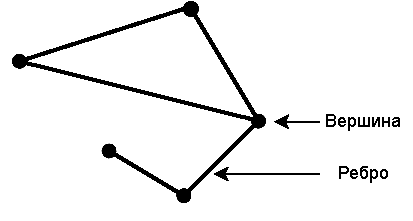
\includegraphics[width=0.4\linewidth]{net.pdf}
	\caption{Пример сети.} 
    \label{p1}
    \end {center}
\end{figure}

\begin{itemize}
    \item Ячеистая (mesh) - каждое устройство подключается к другому устройству через определенный канал;
    \item Топология шины - к коаксиальному кабелю, который выступает в качестве общей разделяемой среды передачи данных подключены все устройства;
    \item Кольцевая топология - соединяющие устройства ровно с двумя соседними устройствами, образуют кольцо;
    \item Топология звезды - все устройства подключаются к одному сетевому устройству через кабель;
    \item Топология дерева - разновидность топологии звезда;
    \item Гибридная топология - комбинация различных топологий;
\end{itemize}
В данной работе мы будем изучать mesh-сети.
\subsection{Mesh-сети}
Как уже было упомянуто в mesh-сети все устройства связаны друг с другом через определенный канал.
Mesh-сети бывают: 
\begin{itemize}
    \item Полносвязными (full mesh);
    \item Неполносвязными (partial mesh).
\end{itemize}

\begin{figure}[H]
	\begin{center}
	\begin{minipage}[h]{0.45\linewidth}
	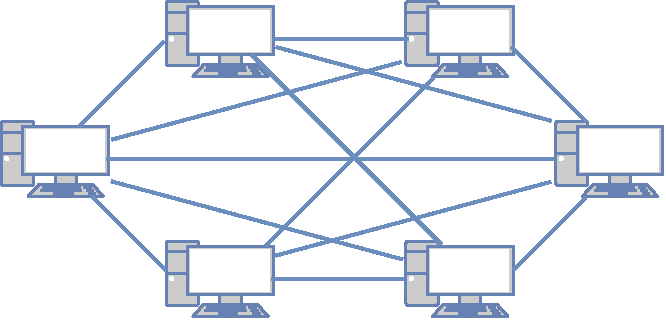
\includegraphics[width=1\linewidth]{full.pdf}
	\caption{Full-mesh сеть.} 
    \label{p2}
	\end{minipage}
	\hfill 
	\begin{minipage}[h]{0.43\linewidth}
	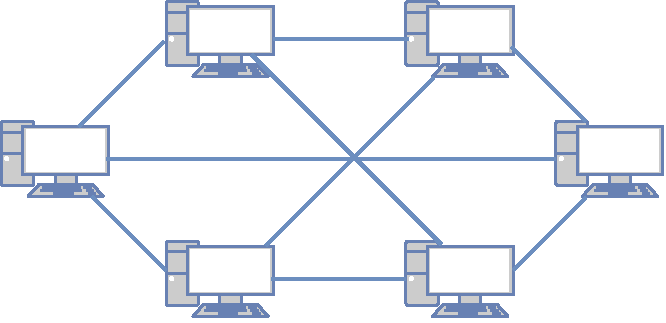
\includegraphics[width=1\linewidth]{partial.pdf}
	\caption{partial-mesh сеть.}
	\label{p3}
	\end{minipage}
	\end{center}
\end{figure}

\textbf{Полноcвязная топология} \par

В данной топологии все узлы в сети связаны друг с другом. Если в сети имеется $N$ узлов, каждый узел будет иметь $N-1$ соединений.
 Полная сетка обеспечивает превосходную степень избыточности, но поскольку ее реализация непомерно дорога, ее обычно резервируют для сетевых магистралей.
 Общее количество ссылок, необходимых для ячеистой топологии, равно $[N(N-1)]/2$.

\textbf{Неполносвязная топология}

Partial mesh сеть более практична по сравнению с full mesh. В частично связанной сетке не все узлы обязательно должны быть связаны друг с другом во время сети. 
Периферийные сети подключаются с использованием частичной сетки и работают в тандеме с полноячеистой сетью.

Топология Mesh основана на децентрализованной схеме организации сети, в отличие от типовых сетей, которые создаются по централизованному принципу.
 Точки доступа, работающие в Mesh-сетях, не только предоставляют услуги абонентского доступа, но и выполняют функции маршрутизаторов/ретрансляторов для других точек доступа той же сети. 

Mesh-сети строятся как совокупность кластеров. Территория покрытия разделяется на кластерные зоны, число которых теоретически не ограничено. 
Особенностью Mesh является использование специальных протоколов, позволяющих каждой точке доступа создавать таблицы абонентов сети с контролем состояния транспортного канала и поддержкой динамической маршрутизации трафика по оптимальному маршруту между соседними точками. 
При отказе какой-либо из них происходит автоматическое перенаправление трафика по другому маршруту, что гарантирует не просто доставку трафика адресату, а доставку за минимальное время.

Процедура расширения сети в пределах кластера ограничивается установкой новых точек доступа, интеграция которых в существующую сеть происходит автоматически.

\subsection{Безопасность Mesh-сетей}

Вопросы безопасности Mesh  являются весьма актуальными, особенно для систем городского масштаба, которые объединяют муниципальные, абонентские и корпоративные сети. 
Безопасность сетей обеспечивается в рамках спецификаций стандарта 802.11. Стандарт IEEE 802.11i предусматривает использование в продуктах Wi-Fi таких средств, как поддержка алгоритмов шифрования трафика: TKIP, WRAP и CCMP.
 Этих алгоритмов достаточно для защиты на уровне абонентского трафика, но на уровне корпоративного пользователя используются дополнительные механизмы, включающие более совершенные способы аутентификации при подключении к сети: более крипто-стойкие методы шифрования, динамическую замену ключей шифрования, использование персональных межсетевых экранов, мониторинг защищенности беспроводной сети, технологию виртуальных частных сетей VPN и т.д.

\subsection[]{Преимущества ячеистой топологии}
\begin{itemize}
    \item В случае сбоя одного устройства - сеть продолжит функционировать в том же режиме.
    \item Просто локализовтаь неисправность.
    \item Передача данных более стабильна, потому что сбой не нарушает ее процессов.
    \item Проблем с трафиком нет, так как для каждого компьютера есть выделенная двухточечная связь.
    \item Эта топология обеспечивает несколько путей для достижения цели и соответственно хорошую помехоустойчивость.
    \item Высокая конфиденциальность и безопасность.
    \item Добавление новых устройств не нарушает передачу данных.
\end{itemize}

\subsection[]{Недостатки ячеистой топологии}
\begin{itemize}
    \item Реализация такой сети дороже по сравнению с противоположными сетевыми топологиями, т.е. звездой, шиной, двухточечной топологией.
    \item Требуемая мощность выше, так как все узлы должны оставаться активными все время и распределять нагрузку.
    \item Существует высокий риск избыточных подключений.
    \item Каждый узел требует дополнительных затрат на техническое обслуживание.
\end{itemize}

\section[]{Реализация}
Даная исследователься работы нацелна создание макета обмена данных в группе мобильных агентов, взаимодействующих в mesh-сети обладающей свойствами “малого мира”.
Возможные технологии для реализации модели:
\begin{itemize}
    \item GNS3
    \item Docker
\end{itemize}

\section{Литература}
\begin{thebibliography}{}
    \bibitem{litlink1}  M. E. J. Newman -  \href{https://github.com/julproh/Thesis}{The Structure and Function of Complex Networks}
    \bibitem{litlink2}  Geeks For Geeks -  \href{https://www.geeksforgeeks.org/advantage-and-disadvantage-of-mesh-topology/}{Advantage and Disadvantage of Mesh Topology}
    \bibitem{litlink2}  Осипов И.Е. -  \href{http://lib.tssonline.ru/articles2/fix-op/mesh_seti_techn_prilozh_oborud}{Технологии и средства связи \#4, 2006}
\end{thebibliography}
\end{document}

